% Exercise ID: MAT_P4FUNCOE_4FIN_ANA_006
% Exercise ID: MAT_P4FUNCOE_4FIN_ANA_006
% Module: MÓDULO P4 - Funções | Concept: Função Inversa | Type: Determinação Analítica
% Difficulty: 2/5 (Fácil) | Type: desenvolvimento
% Points: 10 | Time: 10 min
% Tags: inversa, expressao_analitica, calculo
% Author: Professor | Date: 2025-11-18
% Status: active
% Description: Calcular a expressão da inversa de funções simples

\exercicio
Considere a função $g(x)=2x$.

\begin{enumerate}[label=\alph*]
    \item Determine a expressão analítica da função inversa $g^{-1}(x)$.
    
    \vspace{3cm}
    \item Represente graficamente a função $g$ e a sua inversa $g^{-1}$ no mesmo referencial.
    
    \begin{center}
    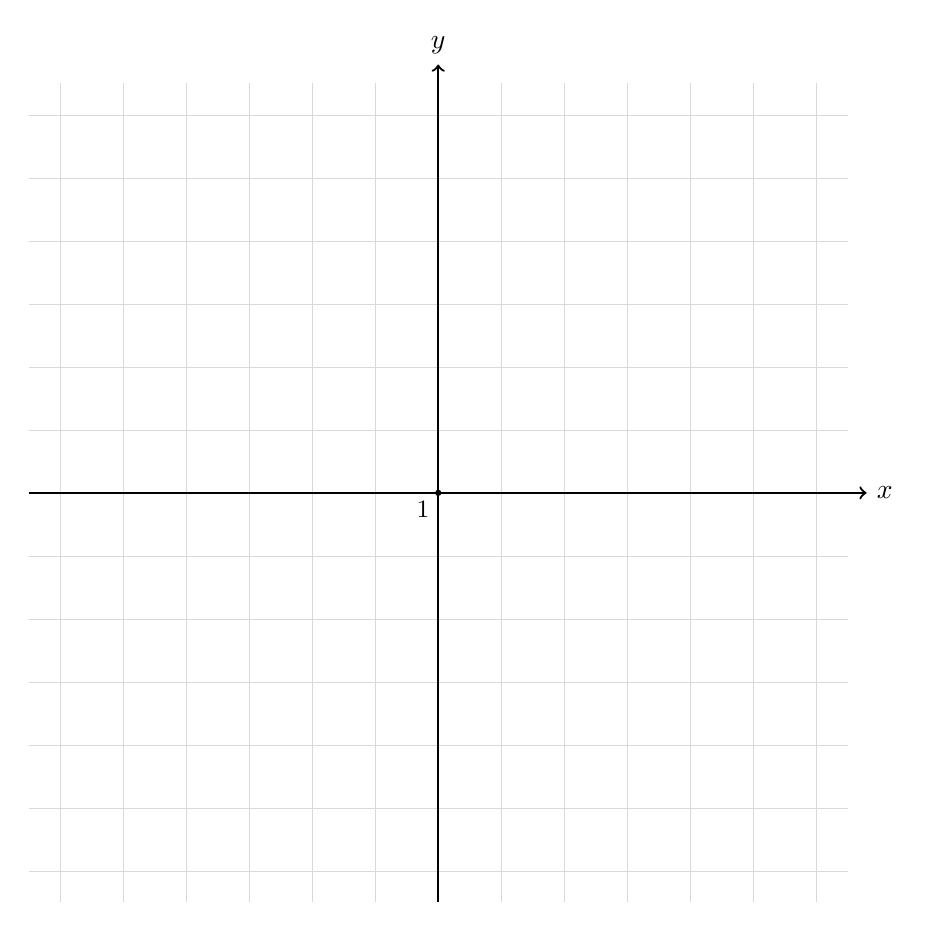
\begin{tikzpicture}[scale=0.8]
        % grid
        \draw[step=1cm,gray!30,very thin] (-6.5,-6.5) grid (6.5,6.5);
        % axes
        \draw[->,thick] (-6.5,0) -- (6.8,0) node[right] {$x$};
        \draw[->,thick] (0,-6.5) -- (0,6.8) node[above] {$y$};
        % origin
        \fill (0,0) circle (0.05) node[below left=2pt,fill=white,inner sep=1pt] {\small $1$};
    \end{tikzpicture}
    \end{center}

\end{enumerate}